%DGraph_counter_example_recovery.tex

\begin{figure*}[c]{0.5\textwidth}
 %   \centering
  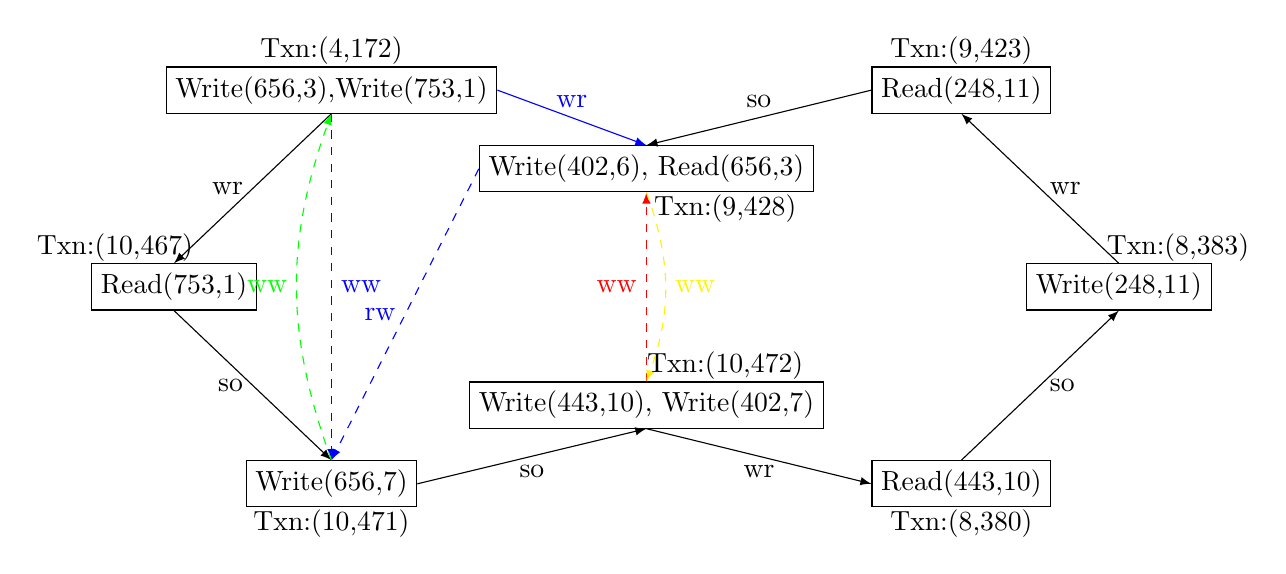
\begin{tikzpicture}[model/.style = {draw, minimum size = 15pt},  node distance = 0.5cm and 1.5cm]
        \node[model] (10472) at (0,0) {Write(443,10), Write(402,7)};
        \node (textof10472) at (1,0.5) {Txn:(10,472)};
        \node[model] (9428) at (0,3) {Write(402,6), Read(656,3)};
        \node (textof9428) at (1,2.5) {Txn:(9,428)};
        \node[model] (10471) at (-4,-1) {Write(656,7)};
        \node (textof10471) at (-4,-1.5) {Txn:(10,471)};
        \node[model] (4172) at (-4,4) {Write(656,3),Write(753,1)};
        \node (textof4172) at (-4,4.5) {Txn:(4,172)};
        \node[model] (10467) at (-6,1.5) {Read(753,1)};
        \node (textof10467) at (-6.75,2) {Txn:(10,467)};
        \node[model] (8380) at (4,-1) {Read(443,10)};
        \node (textof8380) at (4,-1.5) {Txn:(8,380)};
        \node[model] (8383) at (6,1.5) {Write(248,11)};
        \node (textof8383) at (6.75,2) {Txn:(8,383)};
        \node[model] (9423) at (4,4) {Read(248,11)};
        \node (textof9423) at (4,4.5) {Txn:(9,423)};

        
        \path[dashed, -latex, color=red] (10472.north) edge node[left] {ww} (9428.south); 
        \path[dashed, -latex, color=blue] (9428.west) edge node[left] {rw} (10471.north); 
        \path[-latex] (10471.east) edge node[below] {so} (10472.south); 
        \path[-latex, color=blue] (4172.east) edge node[above] {wr} (9428.north) ; 
        \path[-latex] (4172.south) edge node[left] {wr} (10467.north); 
        \path[-latex] (10467.south) edge node[left] {so} (10471.north); 
        \path[-latex] (10472.south) edge node[below] {wr} (8380.west); 
        \path[-latex] (8380.north) edge node[right] {so} (8383.south); 
        \path[-latex] (8383.north) edge node[right] {wr} (9423.south);
        \path[-latex] (9423.west) edge node[above] {so} (9428.north);
        
        \path[dashed, -latex, color=blue] (4172.south) edge node[right] {ww} (10471.north) ; 
        \path[dashed, -latex, color=green] (10471.north)  edge [out=110,in=-110] node[left] {ww}  (4172.south) ; 
        \path[dashed, -latex, color=yellow] (9428.south)  edge [out=-70,in=70] node[right] {ww}  (10472.north) ;
    \end{tikzpicture}
    \caption{Recover the information.}
    \label{fig:recover-DGraph}
\end{figure*}